\documentclass[]{abntex2}
\usepackage{lmodern}	
\usepackage[T1]{fontenc}		
\usepackage[utf8]{inputenc}		
\usepackage{indentfirst}		
\usepackage{nomencl} 			
\usepackage{color}				
\usepackage{graphicx}			
\usepackage{microtype} 			
\usepackage{amsmath}
\usepackage{float}
\usepackage{lipsum}	
\usepackage[brazilian,hyperpageref]{backref}
\usepackage[alf]{abntex2cite}	
\usepackage[table]{xcolor}
\usepackage{amssymb}
\usepackage{hyperref}

\usepackage{listings}
\usepackage{xcolor}

\lstset{
    language=Python,
    basicstyle=\ttfamily\small,
    keywordstyle=\color{blue}\bfseries,
    stringstyle=\color{red},
    commentstyle=\color{gray},
    numbers=left,
    numberstyle=\tiny\color{gray},
    frame=single,
    breaklines=true,
    tabsize=4,
    showspaces=false,
    showstringspaces=false
}

% ---
% Informações de dados para CAPA e FOLHA DE ROSTO
% ---

\titulo{Trabalho - GA030 (Estatística)}
\autor{Lorran de Araújo Durães Soares\thanks{lorranspbr@gmail.com}}
\local{Petrópolis - RJ - Brasil}
\data{2024}
% ---

% ---
% Configurações de aparência do PDF final
% alterando o aspecto da cor azul
\definecolor{blue}{RGB}{41,5,195}
% ---

% Altera as margens padrões
\setlrmarginsandblock{3cm}{3cm}{*}
\setulmarginsandblock{3cm}{3cm}{*}
\checkandfixthelayout

% O tamanho do parágrafo é dado por:
\setlength{\parindent}{1.3cm}

% Controle do espaçamento entre um parágrafo e outro:
\setlength{\parskip}{0.2cm}  % tente também \onelineskip

% Espaçamento simples
\SingleSpacing

\begin{document}

% Retira espaço extra obsoleto entre as frases.
\frenchspacing 

\maketitle

\section*{\textbf{Introdução}}

Este texto refere-se à realização do trabalho da disciplina GA030 (Estatística) do curso de pós graduação do Laboratório Nacional de Computação Científica (LNCC), ministrada pelo prof. Marcio Rentes Borges. Serão apresentadas as questões propostas, seguidas da sua respectiva resolução. \href{https://github.com/lorran-araujo/LNCC/blob/main/disciplinas/estatistica/trab1/trab.ipynb}{Clique aqui} para acessar o código referente à realização de todos os exercícios.

\section*{\textbf{Questão 1}}
\noindent Após abordarmos a \textit{Lei dos Grandes Números} e o \textit{Teorema do Limite Central}, chegamos a um ponto crucial do curso: a estimação de parâmetros (desconhecidos) associados à distribuição de probabilidade de uma variável aleatória.

\noindent O presente trabalho tem como objetivo a fixação das ideias introduzidas até aqui. Para isso, utilizaremos dados armazenados em quatro arquivos, que contêm amostras de diferentes variáveis aleatórias, conforme a Tabela 1.

\begin{table}[H]
    \centering
    \begin{tabular}{|c|c|c|}
        \hline
        \textbf{Variável} & \textbf{Arquivo} & \textbf{Distribuição} \\
        \hline
        $Q \sim \mathcal{N}(0, 2)$ & \texttt{data1q.dat} & Normal \\
        $X \sim U[-1, 1]$ & \texttt{data1x.dat} & Uniforme \\
        $Y \sim E(\lambda = 0.05)$ & \texttt{data1y.dat} & Exponencial \\
        $T \sim B(15, 0.40)$ & \texttt{data1t.dat} & Binomial \\
        \hline
    \end{tabular}
    \caption{Tabela de dados}
    \label{tab:dados}
\end{table}

\section*{\textbf{(a)}}

\noindent Dado que conhecemos a distribuição de probabilidades de cada variável aleatória e os parâmetros que as caracterizam (Tabela \ref{tab:dados}), calcule a expectativa e a variância (teóricas) de cada uma delas, usando as definições que vimos em aula.

\textbf{Resolução:}

Usando as definições dadas em aula e utilizando os parâmetros presentes na tabela \ref{tab:dados}, iremos calcular a média e a variância teórica de cada variável de dados.

\begin{itemize}
    \item Para a variável $Q$, não será necessário cálculos, pois os próprios parâmetros da curva normal fornecem à sua média e variância. Logo, $\mu_Q = 0$ e ${{\sigma}_Q}^{2} = 2$.
    
    \item Para a variável $X$, que tem origem em uma distribuição uniforme, teremos que a média e a variância serão dadas por:
    \[
    \mu_X = \dfrac{-1+1}{2} \Rightarrow \mu_X = 0
    \]
    \[
    {{\sigma}_X}^{2} = \dfrac{{(1-(-1))}^2}{12}=\dfrac{4}{12} \Rightarrow {{\sigma}_X}^{2} = \dfrac{1}{3}
    \]

    \item Para a variável $Y$, originado através de uma distribuição exponencial com $\lambda=0.05$, teremos que a média e a variância serão dadas por:
    \[
    \mu_Y = \dfrac{1}{\lambda} = \dfrac{1}{0.05} \Rightarrow \mu_y = 20
    \]
    \[
    {{\sigma}_Y}^{2} = \dfrac{1}{\lambda^2} = \dfrac{1}{0.05^2} = \dfrac{1}{0.0025} \Rightarrow {{\sigma}_Y}^{2} = 400
    \]

    \item Para a variável $T$, dada por uma distribuição binomial com $p=0.40$ e $N=15$, teremos que a média e a variância serão dadas então por:
    \[
    \mu_T = N \cdot p = 15 \cdot 0.4 \Rightarrow \mu_T = 6
    \]
    \[
    {{\sigma}_T}^{2} = N\cdot p(1-p)=15 \cdot 0.4(1-0.4) \Rightarrow {{\sigma}_T}^{2} = 3.6
    \]
\end{itemize}

Logo, com os resultados obtidos, a tabela \ref{tab:medvar} apresenta a média e variância teóricas de cada uma das variáveis.

\begin{table}[H]
    \centering
    \begin{tabular}{|c|c|c|}
        \hline
        \textbf{Variável} & \textbf{Média} & \textbf{Variância} \\
        \hline
        $Q \sim N(0, 2)$ & $0$ & $2$ \\
        $X \sim U[-1, 1]$ & $0$ & $\dfrac{1}{3}$ \\
        $Y \sim E(\lambda = 0.05)$ & $20$ & $400$ \\
        $T \sim B(15, 0.40)$ & $6$ & $3.6$ \\
        \hline
    \end{tabular}
    \caption{Média e Variância dos dados}
    \label{tab:medvar}
\end{table}

\section*{\textbf{(b)}}

\noindent Utilize o R (ou outro programa) para ler cada arquivo e calcule estimativas para a
média e a variância do conjunto de dados (usando todos os dados disponíveis nos
arquivos). Em seguida, compare com os resultados obtidos no exercício anterior.
Faça comentários.

\textbf{Resolução:}

Para fazer a estimativa da média e da variância de cada variável, iremos usar os estimadores clássicos, pois estes se tratam de estimativas não tendencionas, de variância mínima e coerentes:

\[
\bar{X} = \dfrac{1}{n} \sum_{i=1}^{n} X_i
\]

\[
S^2 = \dfrac{1}{n-1} \sum_{i=1}^{n} (X_i - \bar{X})^2
\]

Foi então construído um programa na linguagem Python, que foi então utilizado para obter as estimativas para a média e para a variância de cada variável aleatória. Os resultados estão presentes na tabela \ref{tab:esti}, apresentadas aqui com três casas decimais de precisão.

\begin{table}[H]
    \centering
    \begin{tabular}{|c|c|c|}
        \hline
        \textbf{Variável} & \textbf{Média} & \textbf{Variância} \\
        \hline
        $Q \sim N(0, 2)$ & $ 0 $ & $2$ \\
        $X \sim U[-1, 1]$ & $0$ & $0.333$ \\
        $Y \sim E(\lambda = 0.05)$ & $20.007$ & $400.37$ \\
        $T \sim B(15, 0.40)$ & $6$ & $3.602$ \\
        \hline
    \end{tabular}
    \caption{Estimativas para a Média e Variância dos dados}
    \label{tab:esti}
\end{table}

Após a realização deste exercício, pode ser observado que as estimativas para a média e para a variância se aproximam consideravelmente dos valores reais. Isso acontece pois o número de amostras de cada conjunto de dados é suficientemente grande. Neste caso, cada variável aleatória possui 5 milhões de amostras, tornando possível estimar a média e a variância com a precisão apresentada.

\section*{\textbf{(c)}}

\noindent Construa os histogramas com as frequências relativas de cada uma das variáveis,
verificando se estes são condizentes com os modelos teóricos (Tabela 1).

\textbf{Resolução:}

Para cada variável, foi construído o histograma das frequências relativas, normalizando os dados para que o histograma, dada a grande quantidade de dados, se aproxime da função de densidade de probabilidade (pdf) ou da função de probabilidade (pf) correspondente à distribuição de origem dos dados. Para realizar essa comparação, a pdf ou pf teórica foi sobreposta ao histograma, com o intuito de verificar se este está condizente com o modelo teórico. A figura \ref{fig:hist} apresenta o resultado obtido. Para as variáveis contínuas, as partições (bins) foram ajustados automaticamente.

\begin{figure}[H]
    \centering 
    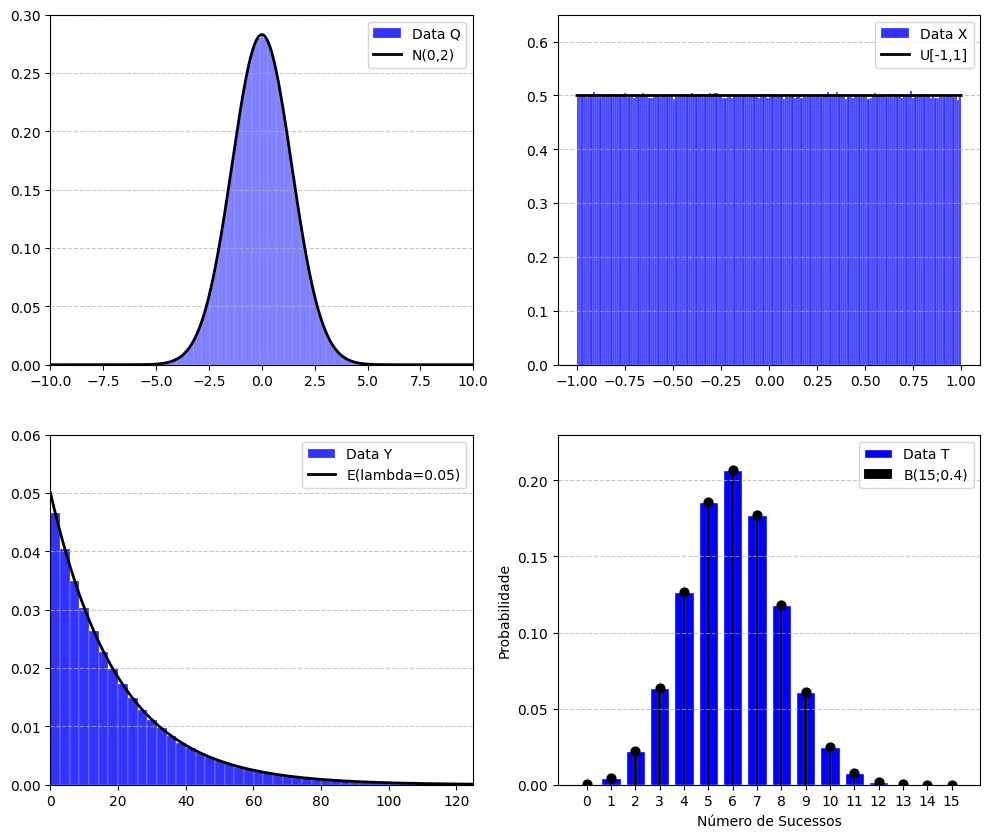
\includegraphics[width=0.8\textwidth]{imgs/hist.png}
    \caption{Histograma de frequências relativas dos dados com distribuições sobrepostas}
    \label{fig:hist} % cria um rótulo para referência no texto
\end{figure}

A visualização da figura acima evidencia que os histogramas estão condizentes com os respectivos modelos teóricos, pois os dados ficaram bem ajustados às respectivas pdf ou pf em todos os casos.

\section*{\textbf{(d)}}

\noindent Considere cada uma das amostras das variáveis aleatórias, contidas nos arquivos, e suas diferentes distribuições de probabilidades. Tome amostras aleatórias de tamanho n (n = 5, 10 e 50) de cada uma das variáveis aleatórias e construa as variáveis aleatórias (estatísticas):

\begin{itemize}
    \item \textit{média amostral:} \[{\bar{W}}^{(n)}=\dfrac{1}{n} \sum_{i=1}^{n} W_i\]
    \item \textit{variância amostral:} \[{S_W}^{2(n)}=\dfrac{1}{n-1} \sum_{i=1}^{n}(W_i - \bar{W}_n)^2\]
\end{itemize}

onde $W = Q, X, Y$ ou $T$. Use 10000 amostras simples (pontos amostrais) para gerar
as variáveis aleatórias média amostral e variância amostral. Obs.: Lembre-se das
características que as amostras aleatórias devem ter. Apresente o código.

\textbf{Resolução:}

Para a realização desta questão, foram realizados 1000 sorteios aleatórios de 5, 10 e posteriormente 50 dados de cada variável, construindo então as variáveis aleatórias média e variância amostrais. A figura \ref{fig:cod} mostra a codificação realizada para a realização desta questão.

\begin{figure}[H]
    \centering
    \begin{minipage}{\textwidth}
    \begin{lstlisting}
        n_samples = [5,10,50]
        
        for key, dat in data.items():
            for n in n_samples:
                medias = []
                variancias = []
        
                amostras = np.random.choice(dat, size=(10000, n), replace=False)
                medias = amostras.mean(axis=1)
                variancias = amostras.var(axis=1, ddof=1)
        
                if key == 'data_q':
                    medias_amostrais_q[f'{key}_{n}'] = medias
                    variancias_amostrais_q[f'{key}_{n}'] = variancias
                elif key == 'data_x':
                    medias_amostrais_x[f'{key}_{n}'] = medias
                    variancias_amostrais_x[f'{key}_{n}'] = variancias
                elif key == 'data_y':
                    medias_amostrais_y[f'{key}_{n}'] = medias
                    variancias_amostrais_y[f'{key}_{n}'] = variancias
                elif key == 'data_t':
                    medias_amostrais_t[f'{key}_{n}'] = medias
                    variancias_amostrais_t[f'{key}_{n}'] = variancias
                else:
                    raise(ValueError)
    \end{lstlisting}   
    \end{minipage} 
    \caption{Código para cálculo das variáveis média amostral e variância amostral}
    \label{fig:cod}
\end{figure}


\section*{\textbf{(e)}}

\noindent Usando o código da questão anterior, construa os histogramas de frequências das
variáveis aleatórias média amostral e variância amostral, para os diferentes valores de n e compare com as distribuições teóricas esperadas para estas variáveis.
Faça isso para as variáveis (Q, X, Y e T).

\textbf{Resolução:}

Para esta questão, é esperado que todas as médias amostrais se aproximem de uma curva normal, com mesma média que a variável de origem e com variância igual a da origem dividida por $n$, onde $n$ se trata do número de amostras que caracterizam a média amostral, neste caso, 5, 10 ou 50. Já para a variância, no caso da variável originada da distribuição normal, é esperado que, multiplicada por um fator, ela se caracterize por uma distribuição qui-quadrada, com $n - 1$ graus de liberdade. Para as outras variáveis, não é esperado que a variância amostral se comporte de uma maneira específica.

Logo, foram construídos os histogramas e as curvas sobrepostas esperadas, presentes nas figuras \ref{fig:medvarQ}, \ref{fig:medvarX}, \ref{fig:medvarY} e \ref{fig:medvarT}, onde cada coluna apresenta o histograma da média amostral (azul) e da variância amostral (vermelha) com $n$ igual a 5, 10 e 50, respectivamente.

\begin{figure}
    \centering 
    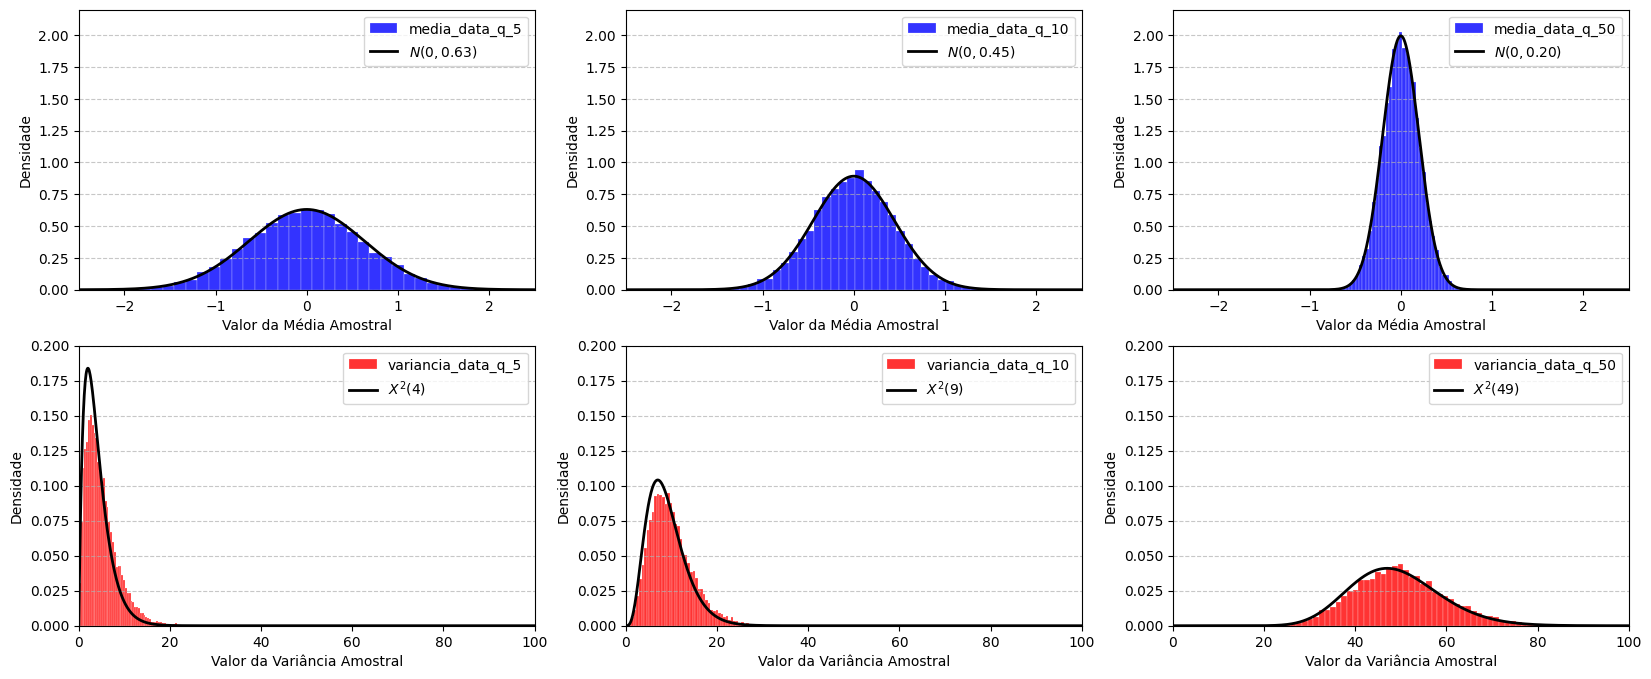
\includegraphics[width=0.95\textwidth]{imgs/medvarQ.png}
    \caption{Histograma das variáveis média e variância amostrais com origem Q}
    \label{fig:medvarQ} % cria um rótulo para referência no texto
\end{figure}

\begin{figure}
    \centering 
    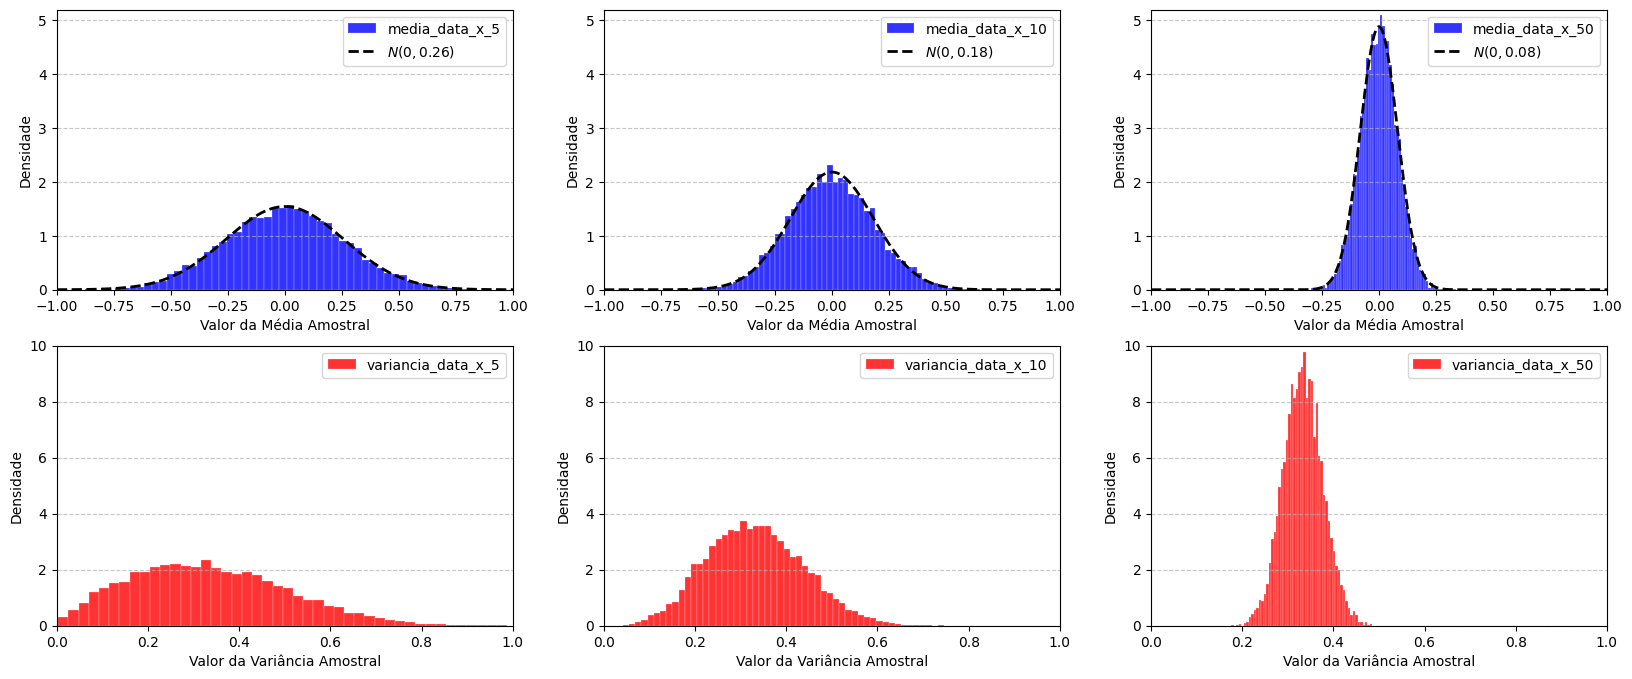
\includegraphics[width=0.95\textwidth]{imgs/medvarX.png}
    \caption{Histograma das variáveis média e variância amostrais com origem X}
    \label{fig:medvarX} % cria um rótulo para referência no texto
\end{figure}

\begin{figure}
    \centering 
    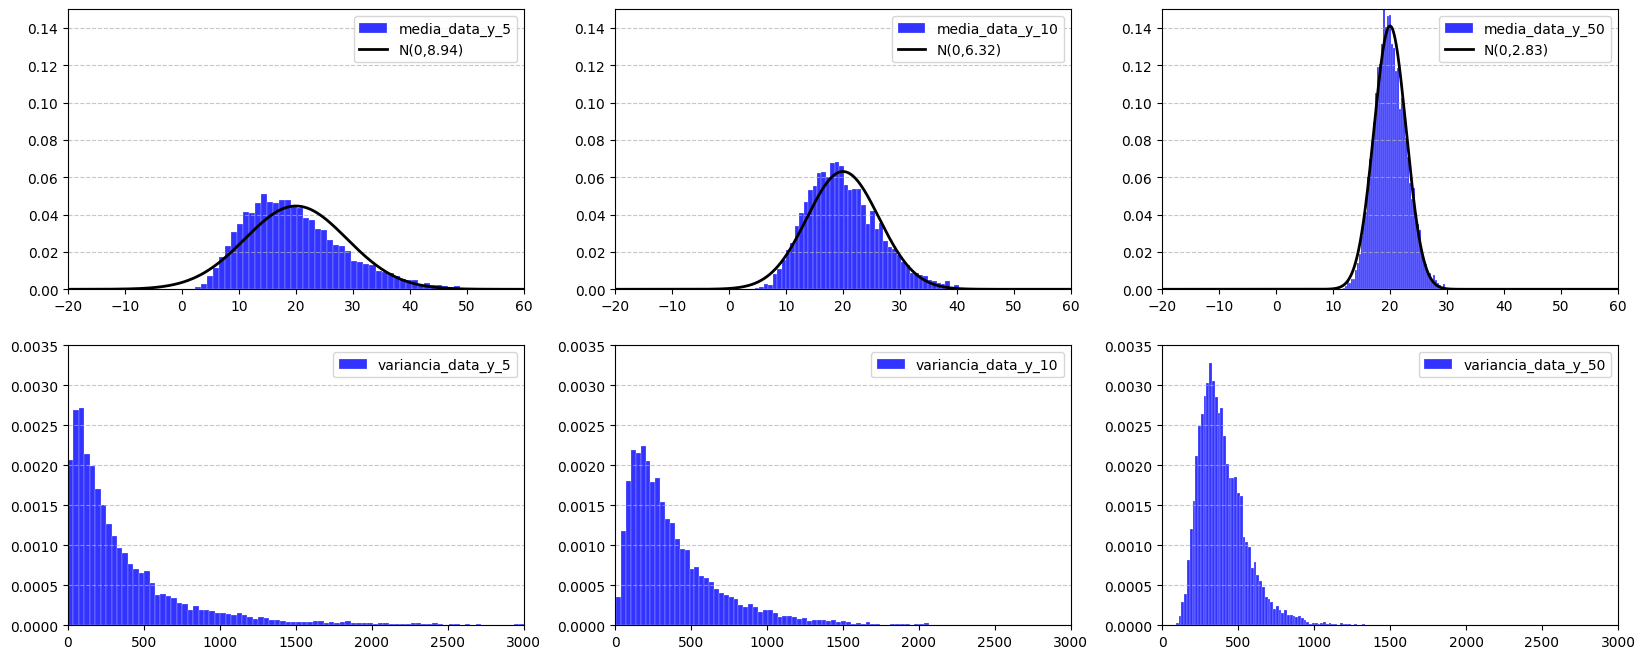
\includegraphics[width=0.95\textwidth]{imgs/medvarY.png}
    \caption{Histograma das variáveis média e variância amostrais  com origem Y}
    \label{fig:medvarY} % cria um rótulo para referência no texto
\end{figure}

\begin{figure}
    \centering 
    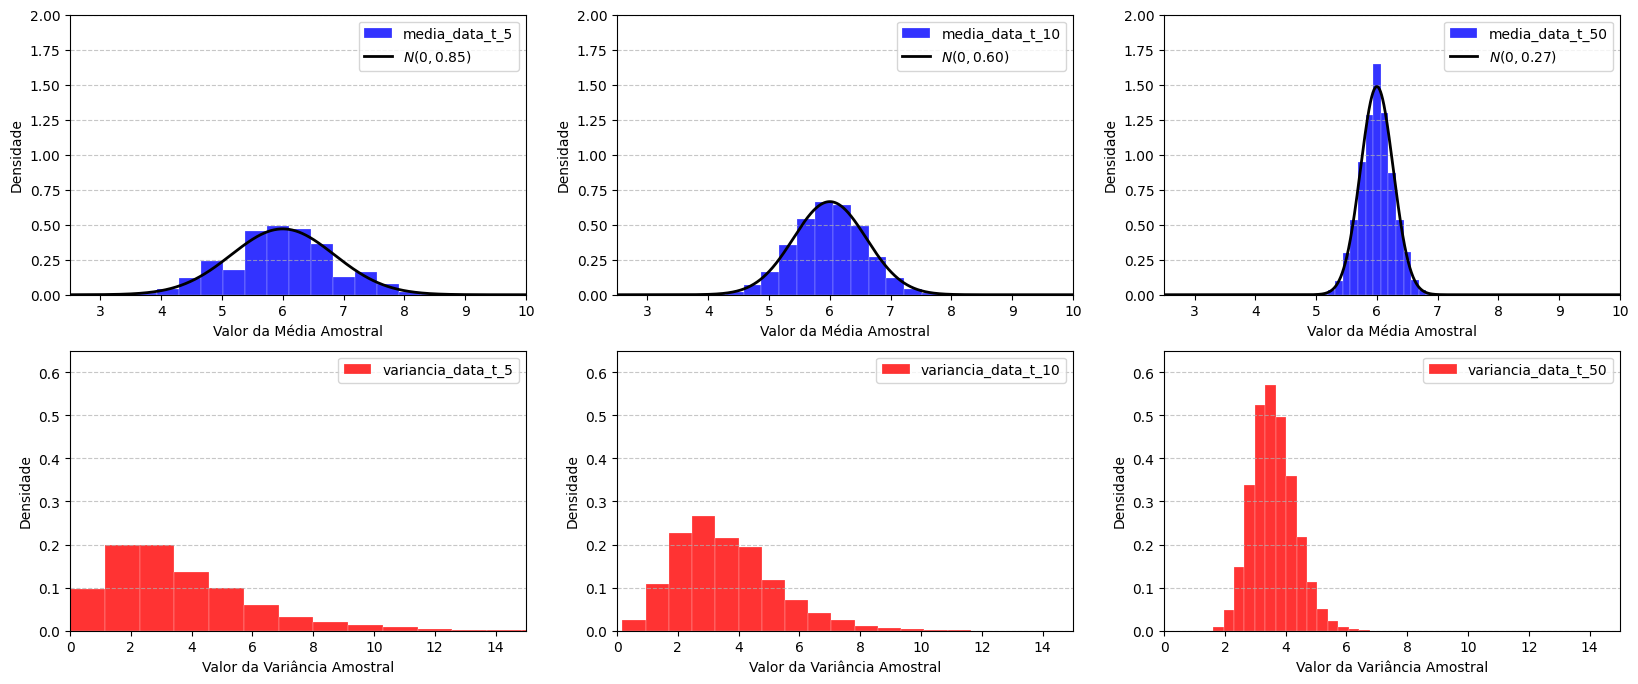
\includegraphics[width=0.95\textwidth]{imgs/medvarT.png}
    \caption{Histograma das variáveis média e variância amostrais com origem T}
    \label{fig:medvarT} % cria um rótulo para referência no texto
\end{figure}

Observando a sobreposição das curvas, pode se notar que os histogramas se aproximam satisfatóriamente das distribuições teóricas esperadas para cada variável.

\section*{\textbf{(e)}}

\noindent Compare os histogramas, para os diferentes valores de n, e discuta os resultados.

\textbf{Resolução:}

Observando as figuras, pode se concluir que quanto maior era a amostra, mais facilmente o histograma se ajustou à sobreposição da curva esperada. Embora não se esperasse nada das outras variâncias, elas também obtiveram uma distribuição blabla parecendo normal e tals.

% ----------------------------------------------------------
% ELEMENTOS PÓS-TEXTUAIS
% ----------------------------------------------------------
\postextual

% ----------------------------------------------------------
% Referências bibliográficas
% ----------------------------------------------------------
\bibliography{Bibliografia}

\end{document}
